\achapter

\answer $v_{1}^{\prime}=\dfrac{\dif x}{\dif t^{\prime}}=\dfrac{\dif x}{\dif t} \cdot \dfrac{\dif t}{\dif t^{\prime}}=-\dfrac{v_{1} L}{v_{1}-v_{2}} \ln \Big(\dfrac{v_{2}}{v_{1}}\Big) \times\Big(\dfrac{v_{2}}{v_{1}}\Big)^{t^{\prime}}$

$a_{1}^{\prime}=\dfrac{\dif v_{1}^{\prime}}{\dif t^{\prime}}=-\dfrac{v_{1} L}{v_{1}-v_{2}}-\ln \Big(\dfrac{v_{2}}{v_{1}}\Big) \times \ln \Big(\dfrac{v_{2}}{v_{1}}\Big) \times\Big(\dfrac{v_{2}}{v_{1}}\Big)^{t^{\prime}} $

$x=v_{1} t=\dfrac{v_{1} L}{v_{1}-v_{2}}\Big[1-\Big(\dfrac{v_{2}}{v_{1}}\Big)^{t^{\prime}}\Big]$\\
因此,$ x\mathdash t'$图即正文中图\ref{fig:01.03} 的反转。
\begin{figurex}
    \centering
    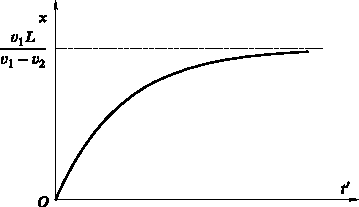
\includegraphics{figure/figa01.01}
    \caption{}
    \label{figa:01.01}
\end{figurex}

\answer (1) 鸟往返了无穷多次

(2) 鸟共飞行了1秒,飞行距离为60公里

(3) $t=\sumx_{h=0}^{t''-1}  \Big(\dfrac{L}{v_{2}+v_{1}}\Big)\Big(\dfrac{v_{2}-v_{1}}{v_{2}+v_{1}}\Big)^{n}$\\
其中$ v_2 $为小鸟速率;$ v_1 $为火车速率

所以得变换为
$    t=\dfrac{2}{3} \sumx_{n=0}^{t'' -1}\Big(\dfrac{1}{3}\Big)^{n}$

\answer $ \Delta s = 5 . 0 2   $米,方向东偏北$ 284^{\circ} $

\answer (1) 位移$ 1.73 $米;路程$ 4.19 $米;平均速度$ D=0.41 $厘米/秒,方向沿
位移方向;瞬时速度为$ v=1.0$厘米/秒,方向沿圆在该点的切线

(2)位移$ 2.0 $米;路程$ 3.14 $米;$ v = 0.64 $厘米/秒,方向沿位移方向
瞬时速度$  v = 1.0 $厘米/秒,方向沿圆在该点的切线方向

\answer (1) $ 61.0 $厘米/秒,$ 60.1 $厘米/秒,$ 60.01 $厘米/秒

(2) $ 60.0 $厘米/秒

(3) $ v = 2 0 t $  , $ a = 2 0  $

\answer (1) $ - 0 .5 $米,$ -0.5 $米/秒

(2) $ 3 $米/秒,$ -6 $米/秒

(3) $ 2.25 $米

(4) $ -9 $米/秒\textsuperscript{2},$ 3 $米/秒\textsuperscript{2},$ -3 $米/秒\textsuperscript{2}

\answer (1) $\sqrt{52}$米/秒

(2) $ 20 $米/秒

\stepcounter{answer}
\answer (1) $ 1 \text{秒差距} = 3 . 0 8 5 7 \times 1 0 ^ { 1 6 } \text{米} = 2 0 6. 2 6 5 \text{AU} = 3 . 2 6 1 6  \text{光年}$

(2) $1 \text{AU} = \dfrac { 1 } { 2 0 6 2 6 5 } \text{秒差距} = 4 . 8 5 \times 1 0 ^ { - 8 } \text{秒差距}$

\answer $ t = 7 . 0   $秒, $ h = 2 4 0   $米

\answer (1) $ 27.4 $公里

(2) $ 166 $秒

\answer (1) $ 2.25 $秒

(2) 两物在地面上相遇,或不会相遇

\answer (1) $ t = 1 . 5   $秒时,$  \alpha = 1 4 ^ { \circ } 4 1 '$; $ t = 2 .  5 $秒时,$  \alpha = - 3 5 ^{\circ} 4 1'  $

(2) 经过$ 0.75 $秒,高度$  h = 1 0 $米

(3) $ R _ { 1 } = 1 0 . 2  $ 米

(4) $ R _ { 2 } = 8 2   $米

\stepcounter{answer}
\answer $ v _ { 0 1 } = 2 2 .  8 $米/秒; $ v _ { 0 2 } = 2 3 . 9 5   $米/秒

\answer (1) $ \alpha = 2 5 ^ { \circ } $  或$6 5 ^ { \circ } $

(2) $ \alpha = 4 5 ^ { \circ } $

\answer (1) 取$ O $为原点,$ x $轴竖直向下,则
$ x = - \dfrac { 1 } { 2 } g t ^ { 2 } $

(2) $ R = v _ { 0 } t  $

\stepcounter{answer}
\answer $ 96 $厘米

\stepcounter{answer}
\answer $ 1.82 $公里

\answer (1) $ 1 6 9   $米/秒

(2) $ 509 $米
(3) 速率$  v = 2 1 0  $ 米/秒,与水平方向夹角$ \alpha = 61^{\circ} $

\answer $ v = \dfrac { n } { 2 } \sqrt { 2 g h }  $

\answer (1) 应沿77°32的纬线自东向西飞行

(2) 可以看见太阳从西向东移动

\answer $ R _ { \text{min} } = 2 2 8   $米

\answer (1) $ \omega = 2 0   $弧度/秒
(2) $ A $点轨迹的参数方程是如下的摆线
\begin{align*}
    x &= r \left( \omega t - \sin \omega t \right)  \\
    y &= r \left( 1 - \cos \omega t \right) \\
    v &= 0 . 5  \text{米} \\
    \omega &= 2 0 \text{弧度/秒}
\end{align*}

\answer (1) 球心速度v与球滚动的角速度a的关系为
\begin{equation*}
    v = \omega \sqrt { r ^ { 2 } - \left( d \operatorname{/} { { 2 } } \right) ^ { 2 } }
\end{equation*}

(2) 球面上任一点的轨迹均为摆线
